% @suppress InvalidSymbol
\section{本研究のシステム}
本研究では兎澤の研究で挙げられていた全体的な認証成功率の低さ,特に手首を中心とする動きの小さいモーションでの認証成功率の改善を目標とする.
また,特定の図形や記号を元にしたモーションだけでなく,端末を上下に振るなどより単純で日常的な入力が容易なモーションでの利用が可能なシステムを目指す.
システムの動作フローを図\ref{flow}に示す.

\begin{figure}[bthp]
    \centering
    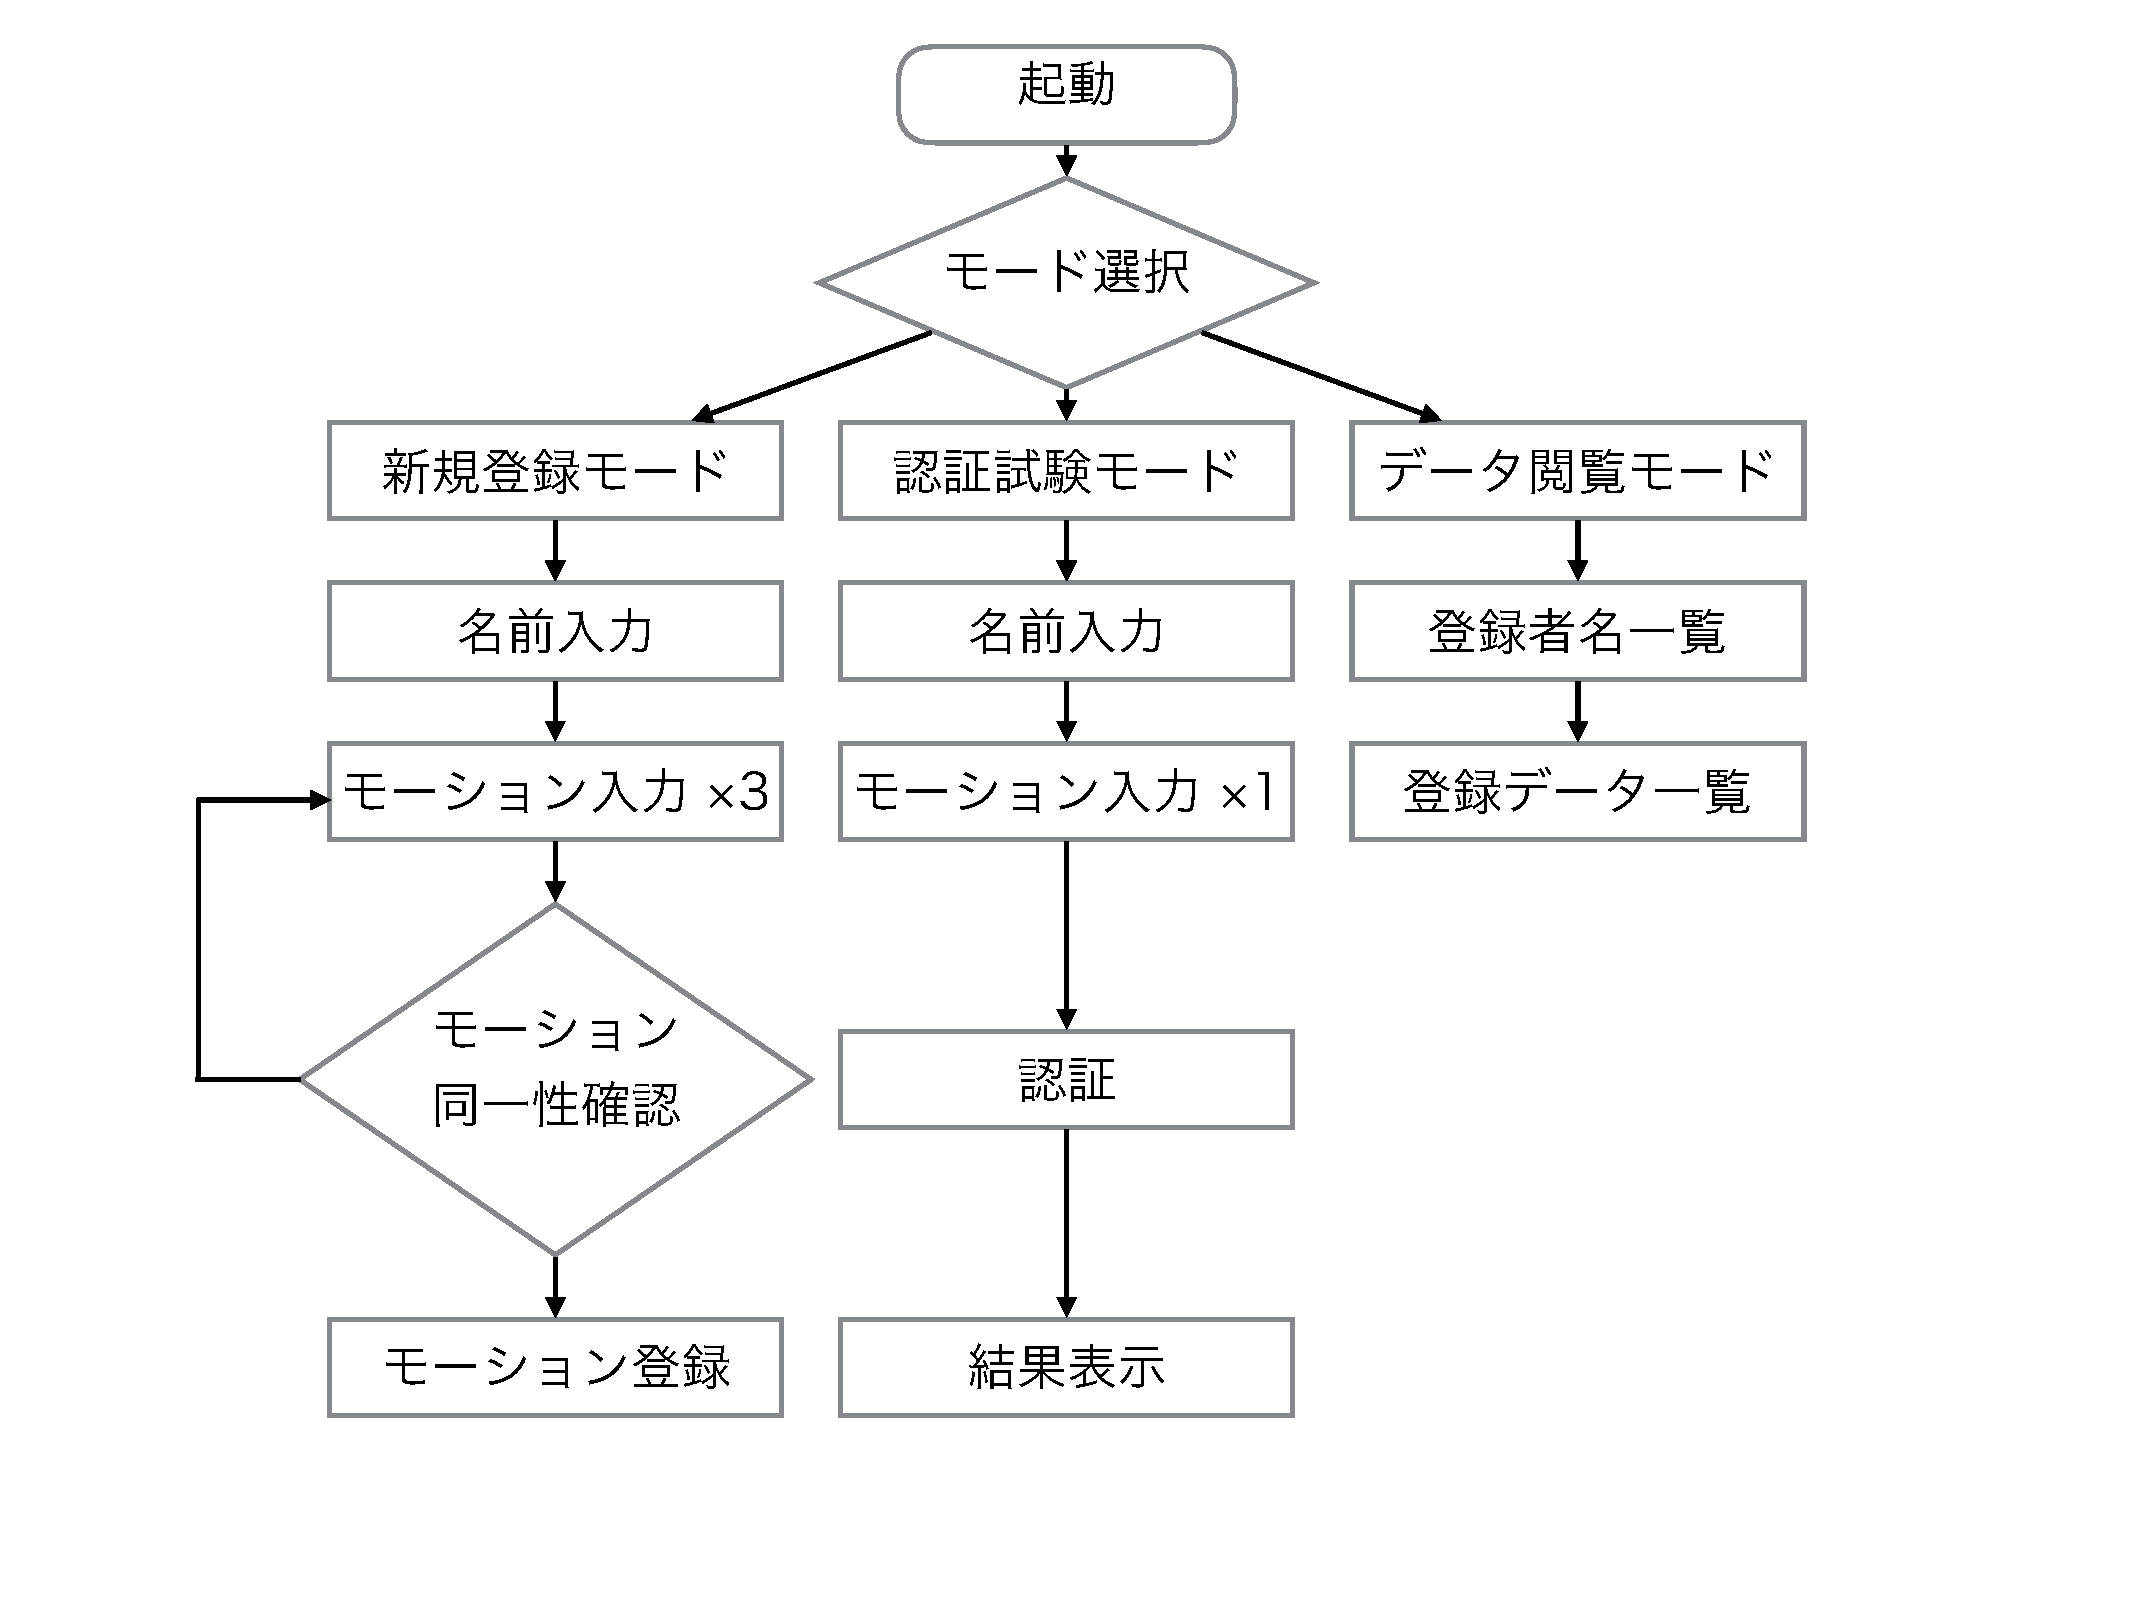
\includegraphics[bb=0 100 950 750, width=80mm]{flow.pdf}
    \caption{システム動作フロー}
    \label{flow}
\end{figure}

アプリケーション起動時に表示されるモード選択ダイアログから,ユーザはまず新規登録モードを選択する.
このモードでは,ユーザ名を指定して個人認証を行う際の鍵情報となるモーションを登録できる.
モード選択後登録したいユーザ名を入力し,モーションの入力を任意の長さで3回行う.
データを取得した後に最も入力時間の長かったデータを基準に他のデータの末尾にゼロを補填する方法でデータの長さを揃え,その後データの振れ幅を確認する.
あらかじめ設定しておいた増幅器の閾値を元に,取得したデータの振れ幅が下回った場合はモーションの動きが小さいとし,全てのデータに増幅量を掛けることで振れ幅の増幅処理を行う.
次にフーリエ変換を用いたローパスフィルタ処理によって,モーション入力時の手の震えなどから生じうるデータへの影響を取り除く.
ローパスフィルタ処理が終われば加速度データから距離を,角速度データから角度を求め,コサイン類似度を用いて取得したデータが同一のモーションであるかを確認する.
同一のモーションであればモーション入力時に生じうる時間的なズレを修正する.
同一のモーションでなければモーションの取り直しを行う.
時間的なズレを修正する処理が終われば処理を行った3回分のデータから平均値を求め,これを増幅量とともに登録する.

これらの処理を行うことで,兎澤の研究であげられていた認証成功率の低さや対応できるモーションに限りがあるという問題に対処している.

認証試験モードでは,あらかじめ新規登録モードにおいてモーションの登録を行ったユーザ名を指定する.
指定されたユーザ名で既にモーションの登録がなされていることが確認できた場合のみ,モーションの入力画面に移る.
認証試験モードでは,モーションの入力を任意の長さで1回行う.
データを取得した後に,登録されたデータの長さを基準にデータの長さが短い場合は末尾にゼロを補填し,長い場合は末尾を切り落とす方法で揃える.
その後新規登録モードにおいてモーションデータとともに登録された増幅量を元に,取得したデータに対して増幅処理を行う.
そしてフーリエ変換を用いたローパスフィルタ処理を行い,加速度データから距離を,角速度データから角度を求める.
これらの処理によって得られたデータと登録されたデータとのコサイン類似度を求め,個人認証を行う.

データ閲覧モードでは,新規登録モードにおいて登録されたユーザ名及びモーションデータを,リスト形式で閲覧できる.

